% !TEX encoding = UTF-8 Unicode
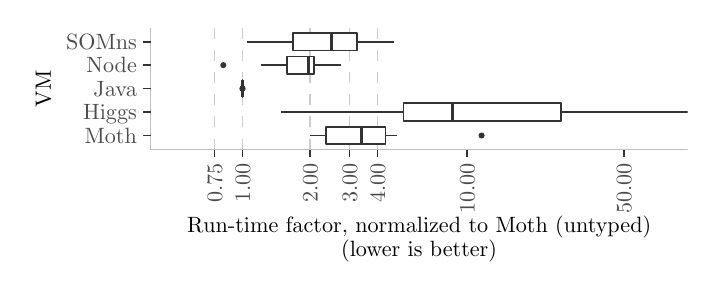
\begin{tikzpicture}[x=1pt,y=1pt]
\definecolor{fillColor}{RGB}{255,255,255}
\path[use as bounding box,fill=fillColor,fill opacity=0.00] (0,0) rectangle (238.49, 86.72);
\begin{scope}
\path[clip] ( 44.40, 42.66) rectangle (238.49, 86.72);
\definecolor{drawColor}{gray}{0.80}

\path[draw=drawColor,line width= 0.6pt,dash pattern=on 4pt off 4pt ,line join=round] ( 67.50, 42.66) -- ( 67.50, 86.72);

\path[draw=drawColor,line width= 0.6pt,dash pattern=on 4pt off 4pt ,line join=round] ( 77.63, 42.66) -- ( 77.63, 86.72);

\path[draw=drawColor,line width= 0.6pt,dash pattern=on 4pt off 4pt ,line join=round] (102.04, 42.66) -- (102.04, 86.72);

\path[draw=drawColor,line width= 0.6pt,dash pattern=on 4pt off 4pt ,line join=round] (116.32, 42.66) -- (116.32, 86.72);

\path[draw=drawColor,line width= 0.6pt,dash pattern=on 4pt off 4pt ,line join=round] (126.45, 42.66) -- (126.45, 86.72);
\definecolor{drawColor}{gray}{0.20}
\definecolor{fillColor}{gray}{0.20}

\path[draw=drawColor,line width= 0.4pt,line join=round,line cap=round,fill=fillColor] (164.01, 47.75) circle (  0.89);

\path[draw=drawColor,line width= 0.6pt,line join=round] (129.32, 47.75) -- (133.51, 47.75);

\path[draw=drawColor,line width= 0.6pt,line join=round] (107.75, 47.75) -- (102.10, 47.75);
\definecolor{fillColor}{RGB}{255,255,255}

\path[draw=drawColor,line width= 0.6pt,line join=round,line cap=round,fill=fillColor] (129.32, 44.57) --
	(107.75, 44.57) --
	(107.75, 50.92) --
	(129.32, 50.92) --
	(129.32, 44.57) --
	cycle;

\path[draw=drawColor,line width= 1.1pt,line join=round] (120.63, 44.57) -- (120.63, 50.92);

\path[draw=drawColor,line width= 0.6pt,line join=round] (192.68, 56.22) -- (238.49, 56.22);

\path[draw=drawColor,line width= 0.6pt,line join=round] (135.85, 56.22) -- ( 91.66, 56.22);

\path[draw=drawColor,line width= 0.6pt,line join=round,line cap=round,fill=fillColor] (192.68, 53.04) --
	(135.85, 53.04) --
	(135.85, 59.40) --
	(192.68, 59.40) --
	(192.68, 53.04) --
	cycle;

\path[draw=drawColor,line width= 1.1pt,line join=round] (153.60, 53.04) -- (153.60, 59.40);
\definecolor{fillColor}{gray}{0.20}

\path[draw=drawColor,line width= 0.4pt,line join=round,line cap=round,fill=fillColor] ( 77.63, 64.69) circle (  0.89);

\path[draw=drawColor,line width= 0.4pt,line join=round,line cap=round,fill=fillColor] ( 77.63, 64.69) circle (  0.89);

\path[draw=drawColor,line width= 0.6pt,line join=round] ( 77.63, 64.69) -- ( 77.63, 64.69);

\path[draw=drawColor,line width= 0.6pt,line join=round] ( 77.63, 64.69) -- ( 77.63, 64.69);
\definecolor{fillColor}{RGB}{255,255,255}

\path[draw=drawColor,line width= 0.6pt,line join=round,line cap=round,fill=fillColor] ( 77.63, 61.52) --
	( 77.63, 61.52) --
	( 77.63, 67.87) --
	( 77.63, 67.87) --
	( 77.63, 61.52) --
	cycle;

\path[draw=drawColor,line width= 1.1pt,line join=round] ( 77.63, 61.52) -- ( 77.63, 67.87);
\definecolor{fillColor}{gray}{0.20}

\path[draw=drawColor,line width= 0.4pt,line join=round,line cap=round,fill=fillColor] ( 70.70, 73.17) circle (  0.89);

\path[draw=drawColor,line width= 0.6pt,line join=round] (103.52, 73.17) -- (113.16, 73.17);

\path[draw=drawColor,line width= 0.6pt,line join=round] ( 93.82, 73.17) -- ( 84.14, 73.17);
\definecolor{fillColor}{RGB}{255,255,255}

\path[draw=drawColor,line width= 0.6pt,line join=round,line cap=round,fill=fillColor] (103.52, 69.99) --
	( 93.82, 69.99) --
	( 93.82, 76.34) --
	(103.52, 76.34) --
	(103.52, 69.99) --
	cycle;

\path[draw=drawColor,line width= 1.1pt,line join=round] (101.59, 69.99) -- (101.59, 76.34);

\path[draw=drawColor,line width= 0.6pt,line join=round] (118.97, 81.64) -- (132.43, 81.64);

\path[draw=drawColor,line width= 0.6pt,line join=round] ( 95.89, 81.64) -- ( 79.30, 81.64);

\path[draw=drawColor,line width= 0.6pt,line join=round,line cap=round,fill=fillColor] (118.97, 78.46) --
	( 95.89, 78.46) --
	( 95.89, 84.82) --
	(118.97, 84.82) --
	(118.97, 78.46) --
	cycle;

\path[draw=drawColor,line width= 1.1pt,line join=round] (109.75, 78.46) -- (109.75, 84.82);
\end{scope}
\begin{scope}
\path[clip] (  0.00,  0.00) rectangle (238.49, 86.72);
\definecolor{drawColor}{RGB}{190,190,190}

\path[draw=drawColor,line width= 0.6pt,line join=round] ( 44.40, 42.66) --
	( 44.40, 86.72);
\end{scope}
\begin{scope}
\path[clip] (  0.00,  0.00) rectangle (238.49, 86.72);
\definecolor{drawColor}{gray}{0.30}

\node[text=drawColor,anchor=base east,inner sep=0pt, outer sep=0pt, scale=  0.80] at ( 39.45, 44.99) {Moth};

\node[text=drawColor,anchor=base east,inner sep=0pt, outer sep=0pt, scale=  0.80] at ( 39.45, 53.46) {Higgs};

\node[text=drawColor,anchor=base east,inner sep=0pt, outer sep=0pt, scale=  0.80] at ( 39.45, 61.94) {Java};

\node[text=drawColor,anchor=base east,inner sep=0pt, outer sep=0pt, scale=  0.80] at ( 39.45, 70.41) {Node};

\node[text=drawColor,anchor=base east,inner sep=0pt, outer sep=0pt, scale=  0.80] at ( 39.45, 78.89) {SOMns};
\end{scope}
\begin{scope}
\path[clip] (  0.00,  0.00) rectangle (238.49, 86.72);
\definecolor{drawColor}{gray}{0.20}

\path[draw=drawColor,line width= 0.6pt,line join=round] ( 41.65, 47.75) --
	( 44.40, 47.75);

\path[draw=drawColor,line width= 0.6pt,line join=round] ( 41.65, 56.22) --
	( 44.40, 56.22);

\path[draw=drawColor,line width= 0.6pt,line join=round] ( 41.65, 64.69) --
	( 44.40, 64.69);

\path[draw=drawColor,line width= 0.6pt,line join=round] ( 41.65, 73.17) --
	( 44.40, 73.17);

\path[draw=drawColor,line width= 0.6pt,line join=round] ( 41.65, 81.64) --
	( 44.40, 81.64);
\end{scope}
\begin{scope}
\path[clip] (  0.00,  0.00) rectangle (238.49, 86.72);
\definecolor{drawColor}{RGB}{190,190,190}

\path[draw=drawColor,line width= 0.6pt,line join=round] ( 44.40, 42.66) --
	(238.49, 42.66);
\end{scope}
\begin{scope}
\path[clip] (  0.00,  0.00) rectangle (238.49, 86.72);
\definecolor{drawColor}{gray}{0.20}

\path[draw=drawColor,line width= 0.6pt,line join=round] ( 67.50, 39.91) --
	( 67.50, 42.66);

\path[draw=drawColor,line width= 0.6pt,line join=round] ( 77.63, 39.91) --
	( 77.63, 42.66);

\path[draw=drawColor,line width= 0.6pt,line join=round] (102.04, 39.91) --
	(102.04, 42.66);

\path[draw=drawColor,line width= 0.6pt,line join=round] (116.32, 39.91) --
	(116.32, 42.66);

\path[draw=drawColor,line width= 0.6pt,line join=round] (126.45, 39.91) --
	(126.45, 42.66);

\path[draw=drawColor,line width= 0.6pt,line join=round] (158.71, 39.91) --
	(158.71, 42.66);

\path[draw=drawColor,line width= 0.6pt,line join=round] (215.39, 39.91) --
	(215.39, 42.66);
\end{scope}
\begin{scope}
\path[clip] (  0.00,  0.00) rectangle (238.49, 86.72);
\definecolor{drawColor}{gray}{0.30}

\node[text=drawColor,rotate= 90.00,anchor=base east,inner sep=0pt, outer sep=0pt, scale=  0.80] at ( 70.25, 37.71) {0.75};

\node[text=drawColor,rotate= 90.00,anchor=base east,inner sep=0pt, outer sep=0pt, scale=  0.80] at ( 80.39, 37.71) {1.00};

\node[text=drawColor,rotate= 90.00,anchor=base east,inner sep=0pt, outer sep=0pt, scale=  0.80] at (104.79, 37.71) {2.00};

\node[text=drawColor,rotate= 90.00,anchor=base east,inner sep=0pt, outer sep=0pt, scale=  0.80] at (119.07, 37.71) {3.00};

\node[text=drawColor,rotate= 90.00,anchor=base east,inner sep=0pt, outer sep=0pt, scale=  0.80] at (129.20, 37.71) {4.00};

\node[text=drawColor,rotate= 90.00,anchor=base east,inner sep=0pt, outer sep=0pt, scale=  0.80] at (161.47, 37.71) {10.00};

\node[text=drawColor,rotate= 90.00,anchor=base east,inner sep=0pt, outer sep=0pt, scale=  0.80] at (218.15, 37.71) {50.00};
\end{scope}
\begin{scope}
\path[clip] (  0.00,  0.00) rectangle (238.49, 86.72);
\definecolor{drawColor}{RGB}{0,0,0}

\node[text=drawColor,anchor=base,inner sep=0pt, outer sep=0pt, scale=  0.80] at (141.44, 12.73) {Run-time factor, normalized to Moth (untyped)};

\node[text=drawColor,anchor=base,inner sep=0pt, outer sep=0pt, scale=  0.80] at (141.44,  4.09) {(lower is better)};
\end{scope}
\begin{scope}
\path[clip] (  0.00,  0.00) rectangle (238.49, 86.72);
\definecolor{drawColor}{RGB}{0,0,0}

\node[text=drawColor,rotate= 90.00,anchor=base,inner sep=0pt, outer sep=0pt, scale=  0.80] at (  8.36, 64.69) {VM};
\end{scope}
\end{tikzpicture}
